\level{1}{Resoconto delle varie attività di verifica - Fase IP}
	Sono riportati in questa appendice tutti i risultati ottenuti nei momenti di verifica, stabiliti nel \insdoc{Piano di Progetto v5.00} secondo la strategia di misurazione per il perseguimento della qualità individuata nel presente documento. Ove fosse necessario, sono state tratte anche delle conclusioni sui risultati ottenuti e su come essi possano essere migliorati.

	\level{2}{Verifica dei prodotti}
		\level{3}{Documenti}
			In questa sezione vengono riportati i risultati delle attività di verifica svolte sui documenti. Esse sono di due tipi:
			\begin{itemize}
				\item verifiche manuali;
				\item verifiche automatizzate.
			\end{itemize}
			\level{4}{Verifiche manuali}
				Le attività di verifica manuale della documentazione prodotta sono state svolte in base alla \insglo{procedura} riguardante la verifica dei documenti che è descritta nel documento \insdoc{Norme di Progetto v5.00}.
				La verifica manuale ha permesso di individuare soprattutto errori riguardanti le seguenti tipologie:
				\begin{itemize}
					\item descrizioni imprecise di classi e metodi;
					\item errori concettuali;
					\item errori nell'utilizzo della lingua inglese.
				\end{itemize}
				Si riporta di seguito la quantità degli errori rilevati e risolti, per ciascuna tipologia, durante l'intera \insglo{fase}.
				\begin{table}[H]
					\centering
						\begin{tabu}{| l | c |}
							\hline
								Descrizioni imprecise	&	8\\ \hline
								Errori concettuali	&	10\\ \hline
								Errori di inglese  &  32\\ \hline
						\end{tabu}
						\caption{Errori trovati tramite verifica manuale dei documenti durante la Fase IP}
				\end{table}
				Si può inoltre notare come gli errori concettuali che sono stati trovati siano in leggera diminuzione, tale fatto ci porta a pensare che i documenti si stanno piano piano avvicinando al loro contenuto ottimale.\\
				Si noti invece come vi sia ancora una notevole quantità di errori nell'uso della lingua inglese imputati alla stesura dei commenti del codice ed alla stesura del documento \insdoc{Manuale utente v2.00}.

	\level{4}{Verifiche automatizzate}
	Le attività di verifica automatizzate sono state effettuate secondo le procedure e attraverso gli strumenti descritti nel documento \insdoc{Norme di Progetto v5.00}. Esse hanno permesso di rilevare diversi errori riguardanti le seguenti tipologie:
	\begin{itemize}
	\item ortografia errata
	\item utilizzo errato dei comandi \LaTeX{} indicati nelle \insdoc{Norme di Progetto v5.00};
	\item norme tipografiche non rispettate.
	\end{itemize}
	Di seguito è presentato un riassunto della quantità di errori trovati (e successivamente risolti) utilizzando la verifica automatica.
	\begin{table}[H]
		\centering
			\begin{tabu}{| l | c |}
				\hline
				Errori ortografici	& 56	\\ \hline
				Utilizzo errato \LaTeX{}	& 0	\\ \hline
				Errori riguardanti norme tipografiche	& 9	\\ \hline
			\end{tabu}
		\caption{Errori trovati tramite verifica automatica dei documenti durante la Fase IP}
	\end{table}

	Risulta evidente come il numero di errori commessi nella redazione sia in continua diminuzione, segno di una maggiore accortezza da parte del gruppo nella redazione delle nuove parti dei documenti, i quali, d'altra parte, si avviano verso la loro versione finale.
	Si riportano i risultati dell'ultima misurazioni dell'indice di leggibilità Gulpease relative ai documenti modificati in questa \insglo{fase}.

	\begin{table}[H]
		\centering
			\begin{tabu}{| l | c | c |}
				\hline
				Documenti 							& Gulpease	& Esito		\\ \hline \hline
				Piano di progetto v5.00				& 87 		& Superato  \\ \hline
				Norme di Progetto v5.00 			& 71		& Superato  \\ \hline
				Piano di Qualifica v5.00 			& 77		& Superato  \\ \hline
				Specifica tecnica v2.00				& 70		& Superato \\ \hline
				Definizione di \insglo{prodotto} v2.00		& 82		& Superato \\ \hline
				Manuale utente v1.00				& 73		& Superato \\ \hline
				Glossario v4.00					 	& 70 		& Superato  \\ \hline
			\end{tabu}
		\caption{Esiti del calcolo dell'indice di leggibilità effettuato tramite strumenti automatici durante la Fase IP}
	\end{table}

	\level{3}{Codice}
	Poichè in questa \insglo{fase} vengono implementate funzionalità desiderabili sfruttando meccanismi estremamente semplici messi a disposizione dalle librerie scelte, molte delle metriche individuate per il codice non sono applicabili, in quanto vengono meno gli oggetti stessi delle misurazioni, quali metodi e classi.
	In questa sezione sono pertanto riportate, per le parti del progetto fino ad ora implementate, i risultati delle metriche calcolati in modo incrementale rispetto alla \insglo{fase} precedente.\\

\level{4}{Numero di requisiti funzionali realizzati}
	\level{5}{Numero di requisiti funzionali obbligatori realizzati}

Si riportano di seguito le percentuali di requisiti funzionali realizzati dalle componenti di \insglo{Norris}.
\begin{table}[H]
	\centering
		\begin{tabu}{| l | c | c |}
			\hline
			Componente	& Percentuale requisiti funzionali obbligatori soddisfatti	& Esito		\\ \hline \hline
			InternalAPIManager	& 100\% 	& Ottimale  \\ \hline
			ExternalAPIManager  & 	96\%	& Accettabile  \\ \hline
			DataModel  & 	100\%	& Ottimale  \\ \hline
		\end{tabu}
	\caption{Esiti del calcolo delle percentuali di requisiti funzionali obbligatori realizzati da Norris durante la Fase IP}
\end{table}
Come è possibile notare dalla tabella la percentuale dei requisiti funzionali obbligatori soddisfatti da \insglo{Norris} ha raggiunto un esito generalmente ottimale. 
\\ \\
Si riportano di seguito le percentuali di requisiti funzionali realizzati dalle componenti di \insglo{Chuck}.
\begin{table}[H]
	\centering
		\begin{tabu}{| l | c | c |}
			\hline
			Componente	& Numero requisiti funzionali obbligatori soddisfatti	& Esito		\\ \hline \hline
			Directive	& 98 \% 	& Ottimale  \\ \hline
			ChartView  & 	99\%	& Ottimale  \\ \hline
			ViewModel  & 	98\%	& Ottimale  \\ \hline
			DataModel  & 	99\%	& Ottimale  \\ \hline
		\end{tabu}
	\caption{Esiti del calcolo delle percentuali di requisiti funzionali obbligatori realizzati da Chuck durante la Fase IP}
\end{table}
Come è possibile notare dalla tabella la percentuale dei requisiti funzionali obbligatori soddisfatti da \insglo{Chuck} ha raggiunto un esito complessivo ottimale.

\level{5}{Numero di requisiti funzionali desiderabili realizzati}

Si riportano di seguito le percentuali di requisiti funzionali realizzati dalle componenti di \insglo{Norris}.
\begin{table}[H]
	\centering
		\begin{tabu}{| l | c | c |}
			\hline
			Componente	& Percentuale requisiti funzionali desiderabilli soddisfatti	& Esito		\\ \hline \hline
			InternalAPIManager	& 81\% 	& Accettabile  \\ \hline
			ExternalAPIManager  & 	83\%	& Accettabile  \\ \hline
			DataModel  & 	100\%	& Ottimale  \\ \hline
		\end{tabu}
	\caption{Esiti del calcolo delle percentuali di requisiti funzionali realizzati da Norris durante la Fase IP}
\end{table}
Come è possibile notare dalla tabella la percentuale dei requisiti funzionali desiderabilli soddisfatti da \insglo{Norris} ha raggiunto un esito generalmente accettabile. 
\\ \\
Si riportano di seguito le percentuali di requisiti funzionali desiderabilli realizzati dalle componenti di \insglo{Chuck}.
\begin{table}[H]
	\centering
		\begin{tabu}{| l | c | c |}
			\hline
			Componente	& Numero requisiti funzionali desiderabilli soddisfatti	& Esito		\\ \hline \hline
			Directive	& 82\% 	& Accettabile  \\ \hline
			ChartView  & 	92\%	& Ottimale  \\ \hline
			ViewModel  & 	87\%	& ottimale  \\ \hline
			DataModel  & 	96\%	& Ottimale  \\ \hline
		\end{tabu}
	\caption{Esiti del calcolo delle percentuali di requisiti funzionali desiderabilli realizzati da Chuck durante la Fase IP}
\end{table}
Come è possibile notare dalla tabella la percentuale dei requisiti funzionali desiderabilli soddisfatti da \insglo{Chuck} ha raggiunto un esito generalmente ottimale.


	\level{2}{Verifica dei processi}

	\level{3}{Processo di documentazione}
	\level{4}{Livello CMM}
	Nonostante i progressi fatti nella capacità di gestione dei processi da parte del gruppo, non è ancora possibile affermare di essere giunti al quarto livello \insglo{CMM}, poichè non è ancora in grado di gestire appieno le misurazioni in un'ottica di miglioramento del processo.

	\level{4}{Schedule Variance}
	Le attività pianificate nel \insdoc{Piano di Progetto v5.00} sono state svolte rispettando le scadenze, senza che si verificasse alcun ritardo significativo.
	Riportiamo di seguito i valori ottenuti calcolando la Schedule Variance sui tempi di stesura di ogni documento:
				\begin{table}[H]
						\centering
						\begin{tabu}{| l | c | c |}
								\hline
								Documenti 							& Schedule Variance	& Esito		\\ \hline \hline
								
								Piano di progetto v5.00				& 0\% 		& Ottimale  \\ \hline
								Norme di Progetto v5.00 			& 1\%		& Ottimale  \\ \hline
								Piano di Qualifica v5.00 			& 2\%		& Ottimale  \\ \hline
								Manuale Utente v2.00 			& 0\%		& Ottimale  \\ \hline
								Definizione di \insglo{Prodotto} v2.00 			& 1\%		& Ottimale  \\ \hline
								Glossario v4.00					 	& 0\% 		& Ottimale  \\ \hline
								Totale processo di documentazione & 4\% & Ottimale \\ \hline
							\end{tabu}
						\caption{Esiti del calcolo della Schedule Variance durante la Fase IP}
					\end{table}
	\level{4}{Budget Variance}
	Le risorse impiegate in questa \insglo{fase} sono risultate essere sovrabbondandanti rispetto alle stime fatte nel \insdoc{Piano di Progetto v5.00}.
	Riportiamo di seguito i valori ottenuti calcolando la Budget Variance sulle risorse utilizzate per la stesura di ogni documento:
				\begin{table}[H]
						\centering
						\begin{tabu}{| l | c | c |}
								\hline
								Documenti 							& Budget Variance	& Esito		\\ \hline \hline
								
								Piano di progetto v5.00				& 0\% 		& Ottimale  \\ \hline
								Norme di Progetto v5.00 			& 1\%		& Ottimale  \\ \hline
								Piano di Qualifica v5.00 			& 1\%		& Ottimale  \\ \hline
								Manuale Utente v2.00  			& 2\%		& Ottimale  \\ \hline
								Definizione di \insglo{Prodotto} v1.00 			& 2\%		& Ottimale  \\ \hline
								Glossario v4.00					 	& 0\% 		& Ottimale  \\ \hline
								Totale processo di documentazione & 6\% & Ottimale \\ \hline
							\end{tabu}
						\caption{Esiti del calcolo della Budget Variance durante la Fase IP}
					\end{table}
	\level{4}{Produttività}
	Utilizzando la formula descritta all'interno del presente documento (sezione \nameref{sec:metriche}) è stata calcolata la produttività del processo di documentazione. Questo indice è stato calcolato durante tutti i momenti di verifica previsti dal \insdoc{Piano di Progetto v5.00} per la \insphase{Fase IP}, e ciò è stato fatto per ogni documento che è stato redatto nel periodo antecedente la verifica. Ogni documento è stato sottoposto al processo di verifica al più cinque volte. Il calcolo fatto di volta in volta sullo stesso documento tiene conto solo delle nuove sezioni introdotte in esso.\\
	Segue un riassunto di quanto è stato fatto.
	\begin{table}[H]
		  \centering
			\begin{tabu}{| l | c | c | c | c | c |}
			\hline
			&1		\\ \hline
			Piano di Progetto	& 156 \\ \hline
			Piano di Qualifica	& 198\\ \hline
			Definizione di \insglo{Prodotto} & 118 \\ \hline
			Manuale Utente & 130	 \\ \hline
			Glossario & 60 \\ \hline
			\end{tabu}
			\caption{Produttività delle varie attività del processo di documentazione durante la Fase IP}
	\end{table}
	Di seguito vengono riportati in un grafico i valori della produttività del processo di documentazione rilevati nei vari periodi della \insphase{Fase IP} nei quali è stato applicato il processo di verifica. Il grafico fa riferimento alla tabella precedente.\\
	% TO DOOOOOOOOOOO!!!!
	\begin{figure}[H]
		\centering
			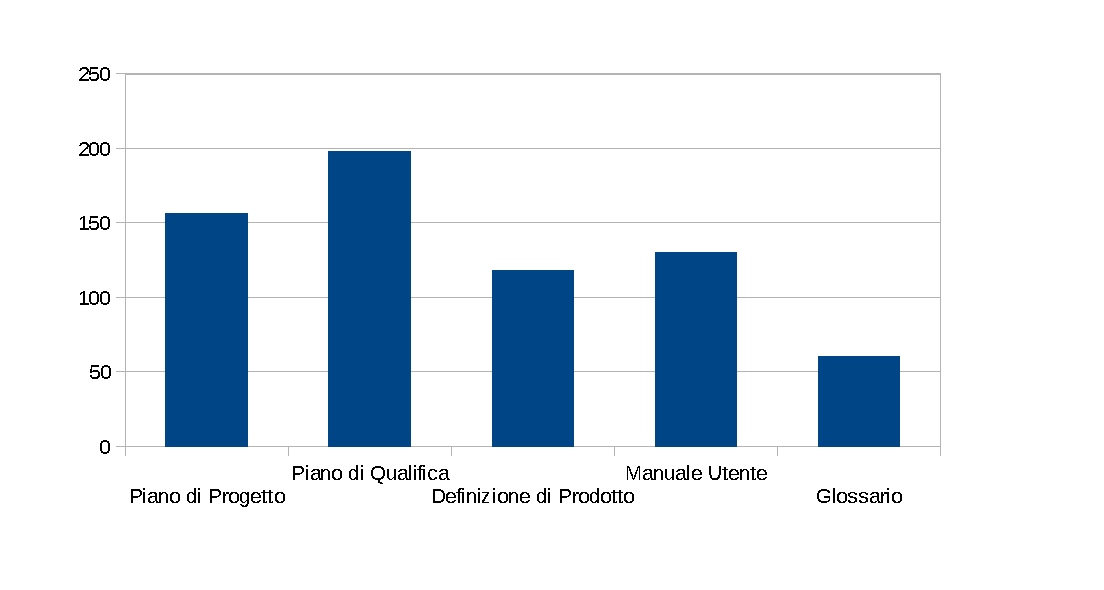
\includegraphics[width=12cm]{PianoDiQualifica/Pics/ProduttivitaDocumentazioneFaseIP.pdf}
		\caption{Produttività del processo di documentazione durante la Fase IP}
	\end{figure}

	Il livello di produttività discretamente alto dei documenti è dovuto al fatto che gli incrementi apportati in questa \insglo{fase} non sono stati particolarmente corposi e non hanno particolari quantità di risorse.

	\level{3}{Processo di verifica}
	\level{4}{Livello CMM}
		Nonostante l'adozione di nuove metriche e una maggiore regolamentazione del processo di verifica, il \insglo{team} non è ancora in grado di individuare miglioramenti tali da comportare un oggettivo aumento della capacità di gestione del processo, necessario per raggiungere il quarto livello \insglo{CMM}, pertanto il processo di verifica rimane al terzo livello (Definito).
	\level{4}{Schedule Variance}
		Il processo di verifica è stato sempre svolto rispettando le scadenze temporali previste nel \insdoc{Piano di Progetto v5.00}. I valori della Schedule Variance calcolati per questo processo risultano quindi ottimi.\\
				Riportiamo di seguito il valore ottenuti:
				\begin{table}[H]
					\centering
					\begin{tabu}{| l | c | c |}
						\hline
							Processi 							& Schedule Variance	& Esito		\\ \hline \hline
							Processo di verifica & 0\% & Ottimale \\ \hline
					\end{tabu}
					\caption{Esiti del calcolo della Schedule Variance durante la Fase IP}
				\end{table}	

	\level{4}{Budget Variance}
	Le risorse utilizzate nel processo di verifica sono risultate leggermente più alte rispetto alle stime del \insdoc{Piano di Progetto v5.00}.
	Riportiamo di seguito il valore ottenuti:
	\begin{table}[H]
		\centering
		\begin{tabu}{| l | c | c |}
		\hline
		Processi 							& Budget Variance	& Esito		\\ \hline \hline
		Processo di verifica & 2\% & Ottimale \\ \hline
		\end{tabu}
		\caption{Esiti del calcolo della Budget Variance durante la Fase IP}
	\end{table}	

	\level{4}{Produttività}
	Utilizzando la formula descritta all'interno del presente documento (sezione \nameref{sec:metriche}) è stata calcolata la produttività del processo di verifica. Tale indice è stato calcolato in seguito a tutti i momenti di verifica previsti dal \insdoc{Piano di Progetto v5.00} per la \insphase{Fase IP}. Di seguito vengono riportati i valori calcolati e una loro rappresentazione grafica.
	\begin{table}[H]
		\centering
		\begin{tabu}{| c | c |}
			\hline
			Data verifica &Produttività\\ \hline \hline
			24/04 & 8 \\ \hline
			29/04 & 12\\ \hline
			01/05 & 5 \\ \hline					
		\end{tabu}
		\caption{Produttività del processo di verifica durante la fase IP}
	\end{table}
	% TO DOOOOOOOOOOO!!!
	\begin{figure}[H]
		\centering
		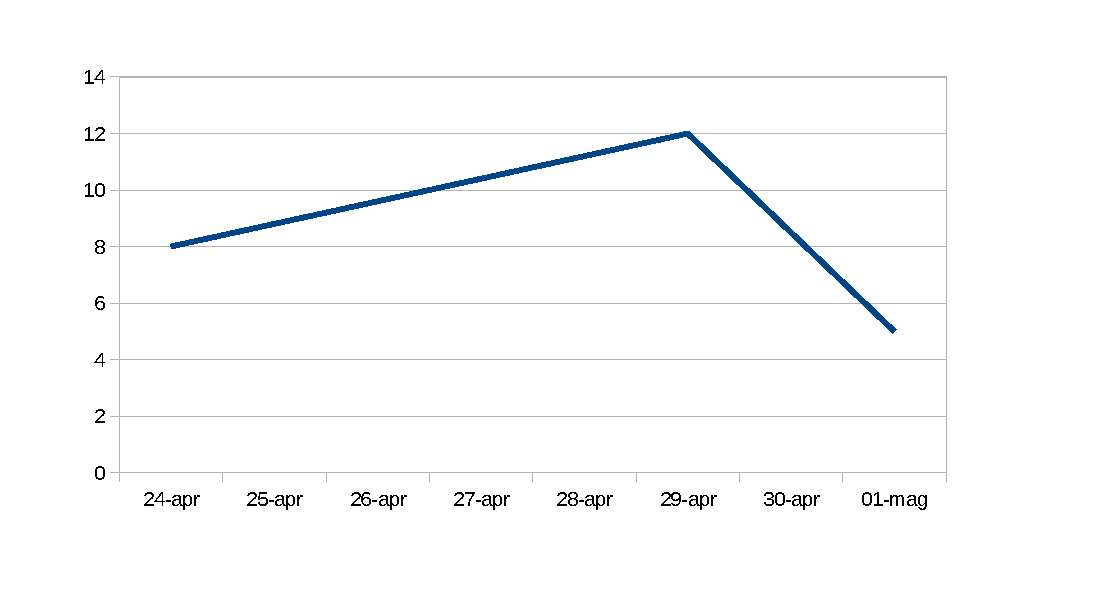
\includegraphics[width=12cm]{PianoDiQualifica/Pics/ProduttivitaVerificaFaseIP.pdf}
		\caption{Produttività del processo di verifica durante la Fase IP}
	\end{figure}

	Si può osservare un aumento di produttività del processo di verifica in corrispondenza del 29 aprile, in quanto in tale data sono stati verificati gli incrementi apportati al \insdoc{Manuale Utente v2.00} e alla \insdoc{Definizione di prodotto v2.00}, entrambi documenti giovani ed incompleti nei contenuti rispetto a quanto previsto per la fine del progetto. Gli altri documenti risultano invece sempre più completi.

	\level{4}{Efficacia di una revisione}
	Utilizzando la formula descritta all'interno del presente documento (sezione \nameref{sec:metriche}) è stata calcolata l'efficacia delle varie revisioni che sono state fatte durante la \insphase{Fase IP}. Di seguito vengono riportati i valori calcolati e una loro rappresentazione grafica.
	\begin{table}[H]
		\centering
		\begin{tabu}{| c | c |}
		\hline
		Data verifica &Efficacia\\ \hline \hline
		24/04 & 6 \\ \hline
		29/04 & 13\\ \hline
		01/05 & 4 \\ \hline		
		\end{tabu}
		\caption{Efficacia delle revisioni durante la fase IP}
	\end{table}
	% TO DOOOOOOOOOOO!!!
	\begin{figure}[H]
		\centering
		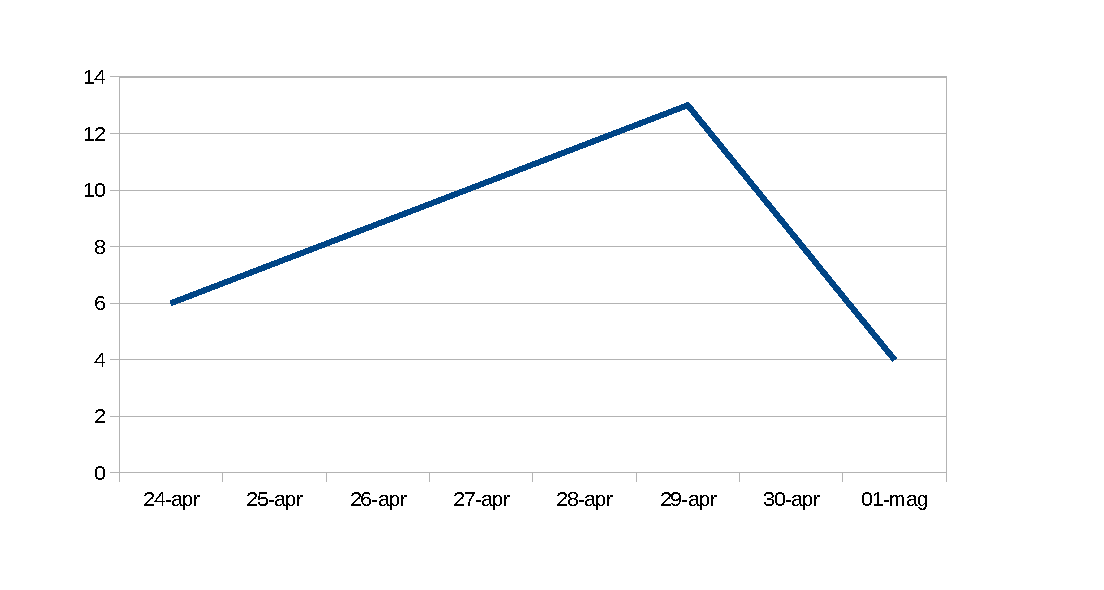
\includegraphics[width=12cm]{PianoDiQualifica/Pics/EfficaciaRevisioniFaseIP.pdf}
		\caption{Efficacia delle revisioni durante la Fase IP}
	\end{figure}

	Correlativamente a quanto detto per la produttività, l'efficacia del processo di verifica in questa \insglo{fase} trova il suo apice nel momento di verifica dei documenti più esposti a possibilità di errore.
	
	\level{3}{Processo di sviluppo}
		Si riportano in questa sezione gli esiti delle misurazioni effettuate rispetto all'attività di codifica.
		\level{4}{Livello CMM}
		In questa \insglo{fase} il livello \insglo{CMM} del processo di sviluppo, relativamente all'attività di codifica, rimane fermo a due. Nonostante i buoni risultati ottenuti, infatti, il \insglo{team} non è in grado di identificare miglioramenti concreti avvenuti nel processo rispetto alla \insglo{fase} precedente.
		
		\level{4}{Schedule Variance}
		Le attività di codifica sono state attuate in anticipo rispetto a quanto previsto nel \insdoc{Piano di Progetto v5.00}.\\
		Riportiamo di seguito i valori ottenuti calcolando la Schedule Variance sui tempi di stesura del codice sorgente.
					\begin{table}[H]
						\centering
						\begin{tabu}{| l | c | c |}
							\hline
								Processi 							& Schedule Variance	& Esito		\\ \hline \hline
								Processo di sviluppo (codifica) & 1\% & Ottimale \\ \hline
						\end{tabu}
						\caption{Esiti del calcolo della Schedule Variance durante la Fase IP}
					\end{table}	
					
		\level{4}{Budget Variance}
		Grazie all'impiego di librerie grafiche estremamente ricche come quelle indicate nella \insdoc{Specifica Tecnica}, utilizzate nello sviluppo del \insglo{prodotto}, le risorse necessarie si sono rivelate leggermente inferiori rispetto alle previsioni.\\
					\begin{table}[H]
						\centering
						\begin{tabu}{| l | c | c |}
							\hline
								Processi 							& Budget Variance	& Esito		\\ \hline \hline
								Processo di sviluppo (codifica) & 2\% & Ottimale \\ \hline
						\end{tabu}
						\caption{Esiti del calcolo della Budgett Variance dell'attività di codifica durante la Fase IP}
					\end{table}	
					
		\level{4}{Produttività}
		Utilizzando la formula descritta all'interno del presente documento (sezione \nameref{sec:metriche}) è stata calcolata la produttività del processo di sviluppo, limitatamente all'attività di codifica. Questo indice è stato calcolato durante i due momenti di verifica previsti dal \insdoc{Piano di Progetto v5.00} per la \insphase{Fase IP}.\\
		Seguono i risultati delle misurazioni.
		\\\begin{table}[H]
						\centering
						\begin{tabu}{| l | c | c |}
							\hline
								Processi 							& 1	& 2		\\ \hline \hline
								Processo di sviluppo (codifica) & 23 & 31  \\ \hline
						\end{tabu}
						\caption{Esiti del calcolo della produttività della codifica durante la Fase IP}
					\end{table}	
		La maggiore produttività registrata nella seconda verifica è dovuta al minor numero di ore impiegate che hanno causato un incremento del rapporto fra quantità di input e output, indice di produttività.

	\level{3}{PDCA}
	In questa sezione viene riportato il grafico \insglo{PDCA} della \insphase{Fase IP}. In ascissa è rappresentato il tempo, in ordinata le attività.
	\begin{figure}[H]
		\centering
		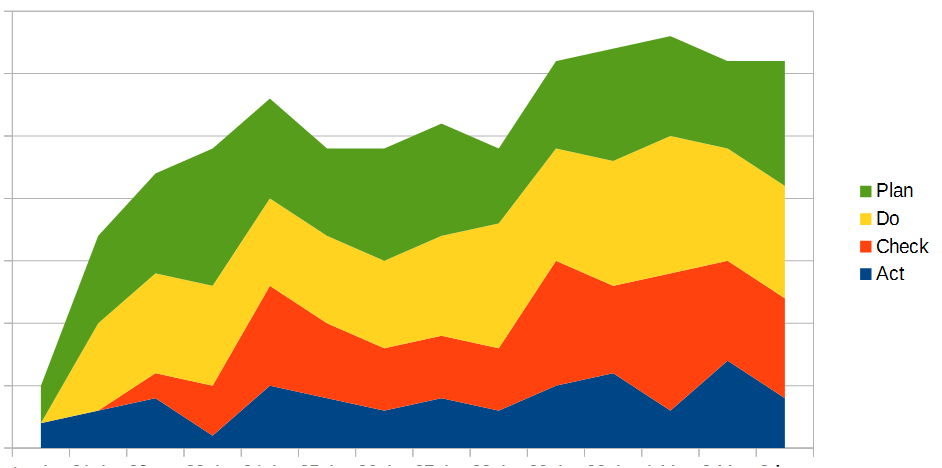
\includegraphics[width=0.6\textwidth]{PianoDiQualifica/Pics/GraficoPDCAFaseIP.png}
		\caption{PDCA Fase IP}
	\end{figure}

	Si può facilmente notare come la pianificazione non abbia subito grossi cambiamenti nel lungo periodo rispetto a quanto si aveva previsto inizialmente. Tale miglioramento è imputabile al lavoro fatto durante le due fasi precedenti che ha reso quasi definitiva la progettazione di \insglo{Norris} e \insglo{Chuck}. Altro aspetto positivo che è facilmente individuabile è il fatto che la pianificazione effettuata dal \insrole{Project Manager} sià stata molto buona per questa \insglo{fase}.